\documentclass[a4paper,12pt]{article}
\usepackage[ngerman]{babel}
\usepackage{graphicx}
\usepackage{color}
\usepackage[utf8]{inputenc}
\usepackage{amsthm}
\usepackage{amsmath}
\usepackage{amssymb}
\usepackage{physics}
\usepackage{enumerate}
\usepackage{siunitx}
\usepackage{hyperref}
\usepackage{pdfpages}
\usepackage{pgfplots}
\usepackage{parskip}
\usepackage{tikz}
\usepackage{bm}
\usepackage{stackengine}
\usepackage{dsfont}
\usepackage{titlesec}
\usepackage{float}
\usepackage{multirow}

% EINIGE COMMANDS

\newcommand{\R}[0]{\mathbb{R}}
\newcommand{\N}[0]{\mathbb{N}}
\newcommand{\C}[0]{\mathbb{C}}
\newcommand{\Z}[0]{\mathbb{Z}}
\newcommand{\Q}[0]{\mathbb{Q}}
\definecolor{lblue}{RGB}{51,153,255} % Farbe für Notizen und besondere Zeichen
\newcommand{\bbew}[0]{\bigg| \bigg|} % Um Endergebnisse doppel zu unterstreichen, außer dass die Striche nicht unten sondern zur Seite stehen
\newcommand{\baro}[0]{\textcolor{lblue}{| }} % Strich um Rechnung von Nebenrechnung/Kommentar zu trennen
\newcommand{\arrowroa}[0]{\textcolor{lblue}{\to}}
\newcommand{\ind}[0]{\ \ \ \ \ }
\newcommand{\indd}[0]{\ind \ind }
\newcommand{\evalint}[3]{\bqty{#1}_{#2}^{#3}} % Stammfunktion mit eckigen Klammern die automatisch auf die entsprechende Größe gesetzt werden
\newcommand{\diff}{\mathrm{\ d}} % d aber nicht in kursiv
\newcommand{\EQ}[0]{\mathrel{\stackon[1pt]{$=$}{$\scriptstyle!$}}} % Gleichheitszeichen mit ! oben drauf
\newcommand{\limit}[2]{\lim\limits_{#1 \to #2}}
\DeclareMathOperator{\Lagr}{\mathcal{L}} % Lagrnaginag
\newcommand{\ELG}[1]{\dv{}{t} \pdv{\Lagr}{\dot{#1}} - \pdv{\Lagr}{#1}} % ELG aber man muss nicht so viel schreiben
\def\tbs{\textbackslash} % backslash but shorter
\newcommand{\e}[1]{\text{e}^{#1}}
\newcommand{\opnorm}[1]{\norm{#1}_{\text{op}}}
\newcommand{\summ}[2]{\sum\limits_{#1}^{#2}}

\newcommand{\mean}[1]{\langle #1 \rangle}

\newcommand{\todo}[1]{\textcolor{red}{TODO: #1}}

\newcommand{\abbref}[1]{Abbildung (\ref{#1})}
\newcommand{\tabref}[1]{Tabelle (\ref{#1})}

\newcommand{\isot}[2]{$^{#1}\mathrm{#2}$}

% EINHEITEN

\newcommand{\gm}[0]{\text{ gm}}
\newcommand{\cm}[0]{\text{\,cm}}
\newcommand{\cmm}[0]{\text{ cm}}
\newcommand{\dm}[0]{\text{ dm}}
\newcommand{\km}[0]{\text{ km}}
\newcommand{\kg}[0]{\text{ kg}}
\newcommand{\m}[0]{\text{ m}}
\newcommand{\s}[0]{\text{ s}}
\newcommand{\J}[0]{\text{ J}}
\newcommand{\Newt}[0]{\text{ N}}
\newcommand{\rad}[0]{\text{ rad}}
\newcommand{\mm}[0]{\text{ mm}}
\newcommand{\mbar}[0]{\text{ mbar}}
\newcommand{\barp}[0]{\text{ bar}}
\newcommand{\mPa}[0]{\text{ mPa}}
\newcommand{\Pa}[0]{\text{ Pa}}
\newcommand{\K}[0]{\text{ K}}
\renewcommand{\l}[0]{\text{ l}}
\newcommand{\mol}[0]{\text{ mol}}
\newcommand{\Mol}[0]{\text{Mol}}
\newcommand{\V}[0]{\text{ V}}
\newcommand{\A}[0]{\text{ A}}
\newcommand{\mA}[0]{\text{ mA}}
\newcommand{\muA}[0]{\ \mu\text{A}}
\newcommand{\Ohm}[0]{\ \Omega}
\newcommand{\kOhm}[0]{\ \text{k}\Omega}
\newcommand{\mOhm}[0]{\ \text{m}\Omega}
\newcommand{\Celsius}[0]{\text{ $^\circ$C}}
\newcommand{\const}[0]{\text{ const.}}

\newcommand{\idf}[0]{\mathrm{id}}

\newcommand{\err}[1]{\Delta #1}
\newcommand{\errpdvsq}[2]{\qty(\pdv{#1}{#2} \cdot \err{#2})^2}
\newcommand{\errsq}[2]{\qty(#1 \cdot \err{#2})^2}
\newcommand{\errsqval}[2]{\qty(#1 \cdot #2)^2}
\newcommand{\errpdv}[2]{\pdv{#1}{#2} \cdot \err{#2}}

\newcommand{\chisq}{\chi^{2}}
\newcommand{\chisqrd}{\chi^{2}_{\mathrm{red}}}

%LA Zeug
\newcommand{\EndVS}[0]{\mathrm{End}} % Endomorphismen
\newcommand{\EigVS}[0]{\mathrm{Eig}} % Eigenraum
\newcommand{\IsomVS}[0]{\mathrm{Isom}} %Isometrien
\newcommand{\Ann}[0]{\mathrm{Ann}} %Annullator
\newcommand{\LinSpan}[0]{\mathrm{Span}} %Linearer Spann
\newcommand{\GL}[0]{\mathrm{GL}} % General Linear Group
\newcommand{\Mat}[3]{\mathrm{Mat}(#1,#2;#3)} % Matritzenraum
\newcommand{\idmat}[0]{\mathds{1}} % einheitsmatrix symbol
\newcommand{\idmatd}[2]{\mathds{1}_{#1 \times #2}} % einheitsmatrix symbol mit suffix
\newcommand{\im}[0]{\mathrm{im}} % Bildraum
\newcommand{\id}[0]{\mathrm{id}} % Identitätsabbildung
\newcommand{\modsp}[2]{{\raisebox{.2em}{$#1$}\left/\raisebox{-.3em}{$#2$}\right.}} % Faktor/Quotient
\newcommand{\longto}[0]{\longrightarrow} %langes äquivalent zu \to
\newcommand{\Hau}[2]{\mathrm{Hau_{#1}\qty(#2)}}

\newcommand{\zz}[0]{Z\kern-.3em\raise-0.5ex\hbox{Z}: } % zu zeigen / z.z.

\newcommand{\ffrac}[2]{\flatfrac{#1}{#2}}
\newcommand{\Thalf}[0]{T_{\flatfrac{1}{2}}}


% MATHEMATISCHE OPERATOREN DIE NICHT IN DEN PACKAGES SIND

\DeclareMathOperator{\arcosh}{arcosh}
\DeclareMathOperator{\acsinh}{arsinh}
\DeclareMathOperator{\artanh}{artanh}
\DeclareMathOperator{\arcsech}{arcsech}
\DeclareMathOperator{\arccsch}{arcCsch}
\DeclareMathOperator{\arccoth}{arcCoth}


\setlength{\textheight}{26cm} \setlength{\footskip}{1cm}
\setlength{\topmargin}{-20mm} \setlength{\headheight}{5mm}
\setlength{\headsep}{5mm} \setlength{\textwidth}{16cm}
\setlength{\evensidemargin}{0mm} \setlength{\oddsidemargin}{0mm}


% NÜTZLICHE TRICKS

% Benutze kein \left( \right), der "physics" package hat \pqty{} (runde Klammern), \bqty{} (eckige Klammern), die die Größe der Klammern automatisch anpassen mehr zum phyisics package hier: http://mirrors.ibiblio.org/CTAN/macros/latex/contrib/physics/physics.pdf

% 


\def\checkmark{\tikz\fill[scale=0.4](0,.35) -- (.25,0) -- (1,.7) -- (.25,.15) -- cycle;} 

\DeclareSIPrePower\quartic{4}
\sisetup{per-mode=fraction}
\sisetup{exponent-product=\cdot}
\renewcommand{\labelenumi}{\alph{enumi})}
\setlength{\parindent}{0pt}
\newcounter{versuchnr}
\newcounter{gruppe}
\allowdisplaybreaks

\titleformat*{\section}{\large\bfseries}
\titleformat*{\subsection}{\normalsize\bfseries}
\titleformat*{\subsubsection}{\normalsize\it}

\renewcommand{\arraystretch}{1.2}





\begin{document}
	
	%%%%%%% Name(n) der Abgebenden
	\newcommand{\name}{Marius Pfeiffer}

	%%%%%%% Daten Versuch
	\setcounter{versuchnr}{255}
	\newcommand{\versuchtitel}{Röntgenspektrometer}
	\newcommand{\protocolpdf}{files/255messprotokoll.pdf}
	\newcommand{\titleimg}{files/versuchsaufbau.png}
	\newcommand{\betreuer}{Valentin Krems}
	\newcommand{\datum}{13.02.2025}
	
	
	\begin{center}
		{Physikalisches Anfängerpraktikum III für Lehramtsstudierende}\\[3mm]
	\end{center}
	
	\vspace*{5mm}
	
	\noindent Name: \name{}
	\hfill Matrikel-Nr.: 4188573\\
	E-Mail: marius.pfeiffer@stud.uni-heidelberg.de
	
	\vspace*{2mm}
	\noindent Betreut durch: \betreuer
    \hfill \datum

	\vspace*{2mm}
	\hrule \vspace*{10mm}

  \begin{center}
    {\bf \large Versuch \arabic{versuchnr}: \it \bf \versuchtitel}
  \end{center}

  \vspace*{10mm}

  \begin{figure}[H]
    \centering
    \includegraphics[width=.8\textwidth]{\titleimg}
    \caption{Versuchsaufbau (Quelle: Praktikumsanleitung).}
  \end{figure}

  \tableofcontents
	\newpage\noindent
	%%%%%%%%%%%%%%%%%%%%%%%%%%%%%%%%%%%%%%%%%%%%%%%%%%%%%%%%%%%%%%%%%%%%%%%%
	\section{Einleitung}
	
	In Versuch 255 setzen wir uns mit der Funktionsweise einer Röntgenröhre, sowie dem charakteristischen Spektrum der Röntenstrahlung auseinander. Neben quantitativen Untersuchungen des Röntgenspektrums selbst, nutzen wir das Prinzip der Bragg-Reflexion, um unter anderem die Gitterkonstante eines NaCl-Kristalls zu bestimmen.

\subsection{Physikalische Grundlagen}

\subsubsection*{Die Röntgenröhre}
Eine Röntgenröhre ist aufgebaut aus einer Glühkathode und einer Anode, welche sich in einem evakuierten Glaskolben befinden. Durch Glühemmission werden aus der Kathode Elektronen freigesetzt, welche durch eine Beschleunigungsspannung von $10$ bis $100\si{\kilo\volt}$, welche zwischen Kathode und Anode anliegt beschleunigt werden. Der kontinuierliche Teil des Röntgenspektrums wird durch die ausgehende Bremsstrahlung beim Abbremsen der Elektronen im Anodenmaterial verursacht. Diese Strahlung setzt bei einer bestimmten Grenzwellenlänge $\lambda_{gr}$ ein, welche sich nach
\begin{align}
  \lambda_{gr} = \frac{hc}{eU}\label{eq:grenzfreq}
\end{align}
berechnen lässt. Hierbei sind $h,c,e$ das Plank'sche Wirkungsquantum, die Lichtgeschwindigkeit und die Elementarladung. $U$ ist die an der Röntgenröhre anliegende Beschleunigungsspannung. Durch frei werdende Strahlung bei der Ionisation des Anodenmaterials ist dem kontinuierlichen Spektrum ein diskretes Spektrum überlagert, zu sehen in \abbref{fig:roentgenspektrum}, welches charakteristisch für das jeweilige Anodenmaterial ist. 

\begin{figure}[H]
  \centering
  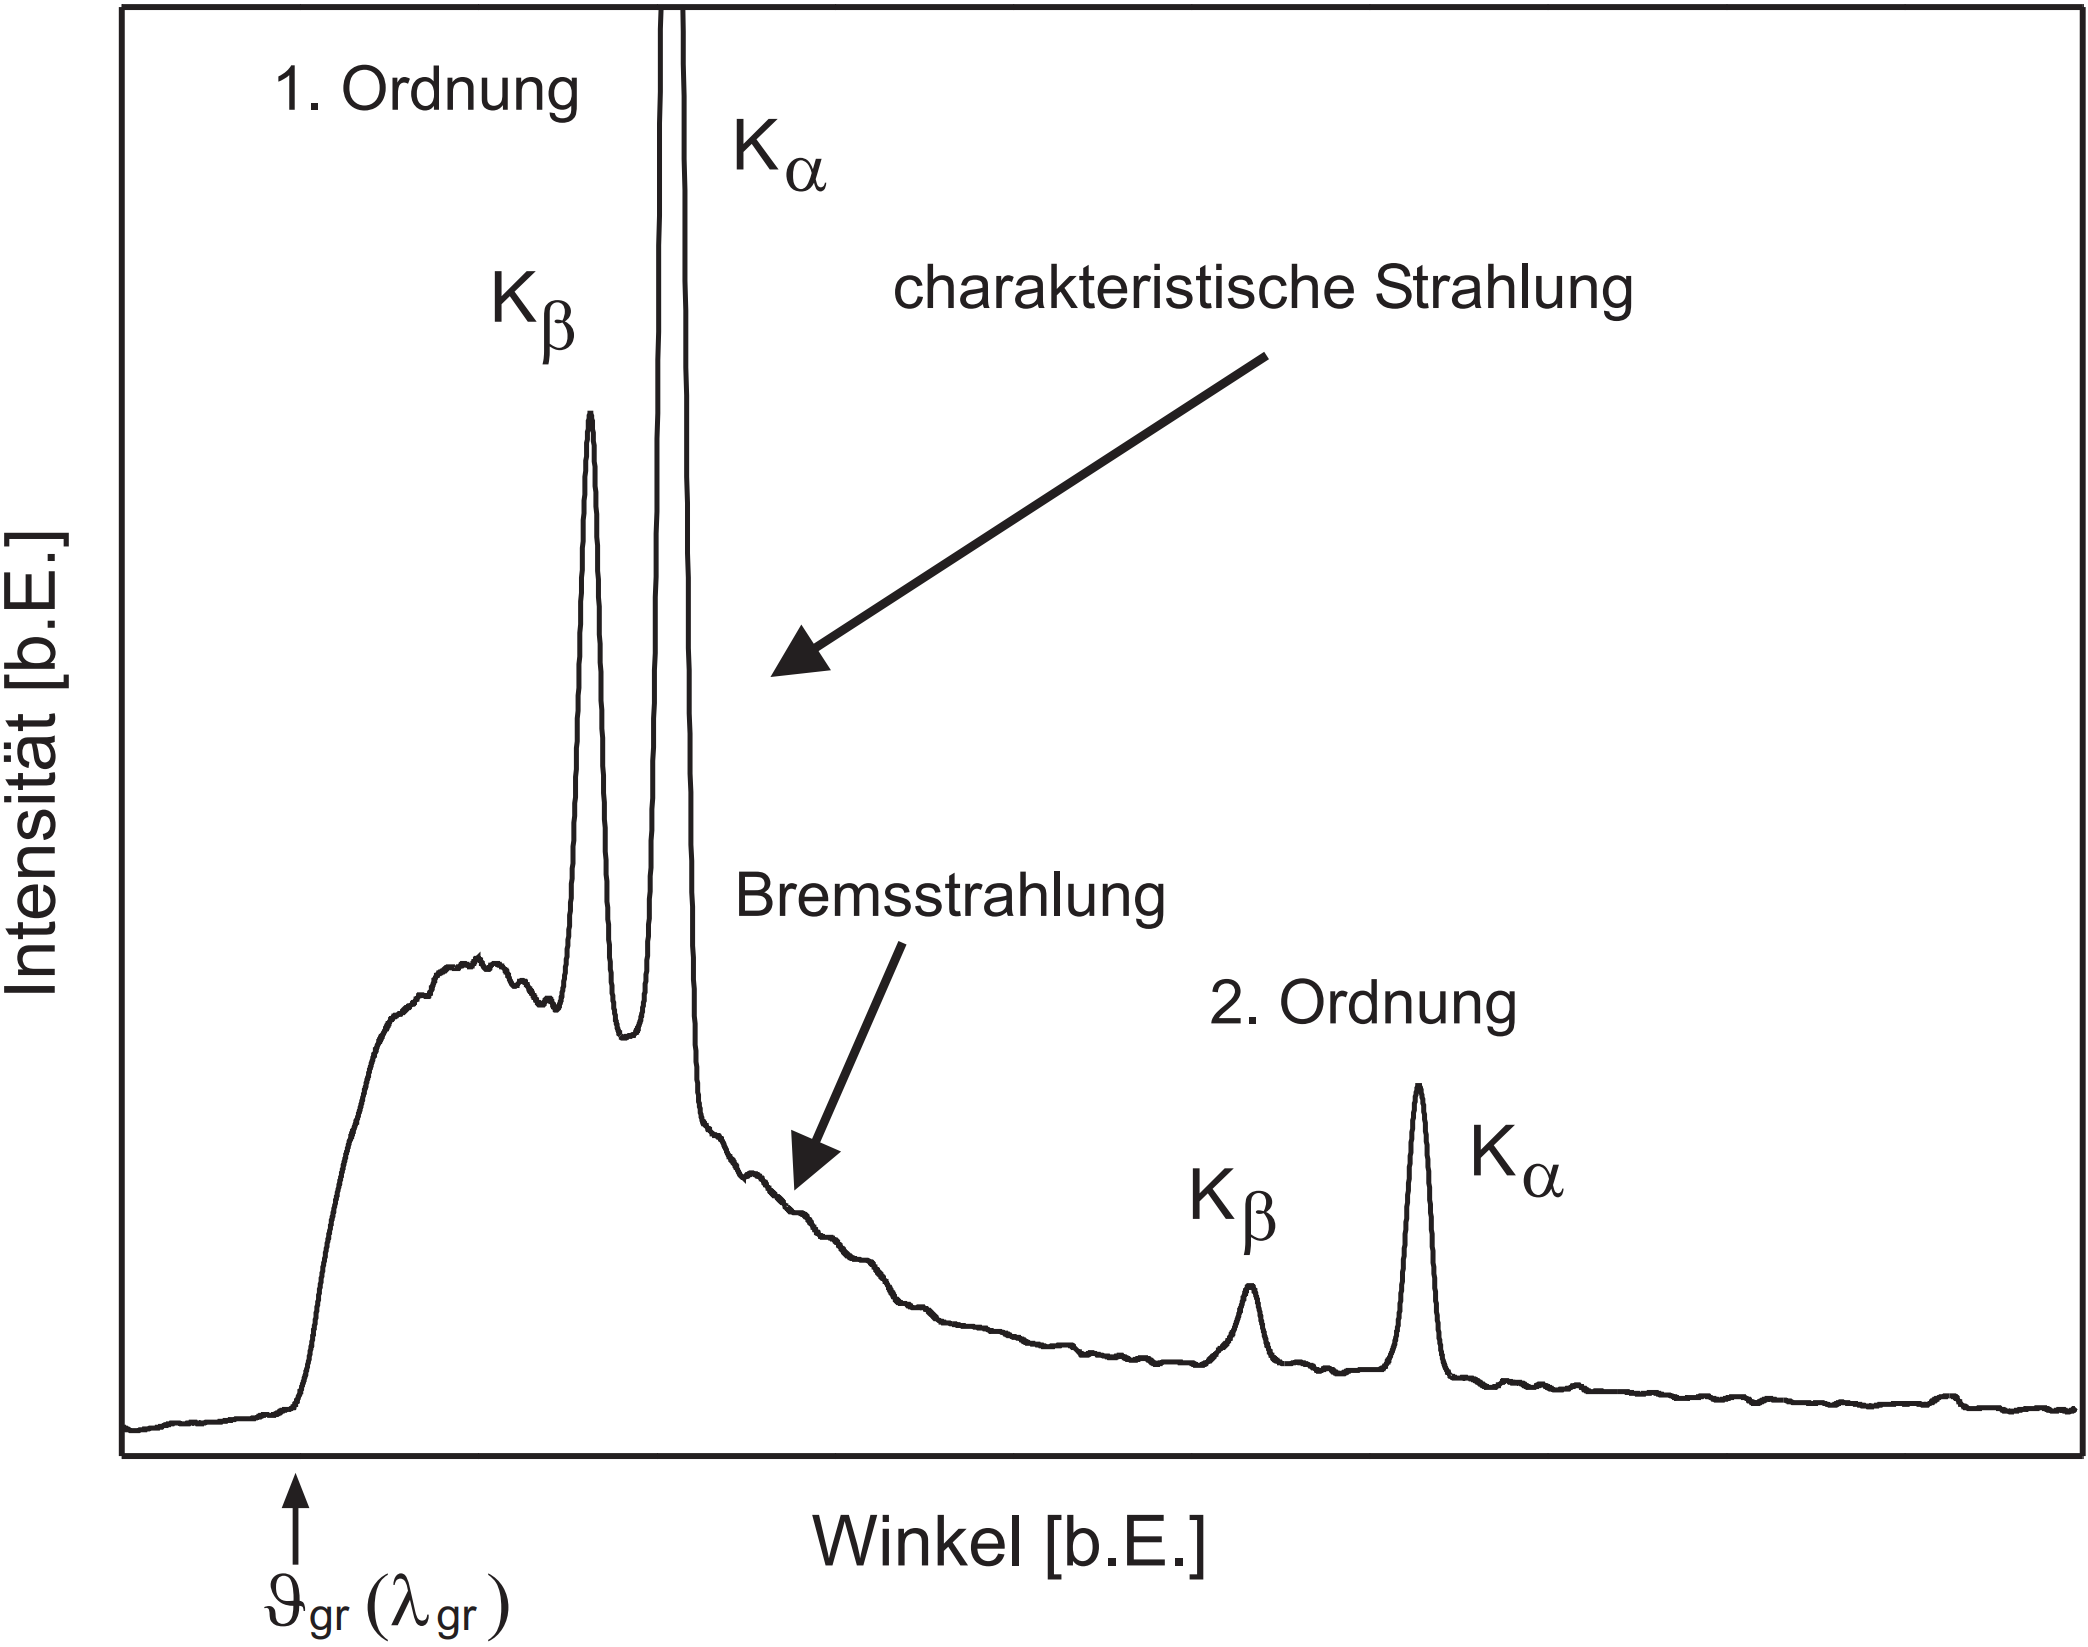
\includegraphics[width=.75\textwidth]{files/roentgenspektrum.png}
  \caption{Kontinuierliches und diskretes Röntgenspektrum.}
  \label{fig:roentgenspektrum}
\end{figure}

Die Positionen der Linien im diskreten Spektrum sind abhängig von der Ursprungs- und Ziel-Schale von bzw. zu welcher der Übergang des Elektrons stattfindet. Beispielsweise bezeichnen wir die Strahlung der Übergänge von der $L$- auf die $K$-Schale als $K_{\alpha}$-Strahlung, die für die Übergänge der $M$- auf die $K$-Schale als $K_{\beta}$-Strahlung. Die freiwerdende Energie eines Übergangs von der $n$-ten zur $m$-ten Schale lässt sich durch das Moseley'sche Gesetz
\begin{align}
  E_{n\to m} = hc R_{\infty} (Z-A)^2 \qty(\frac{1}{m^2} - \frac{1}{n^2})
\end{align}
berechnen. Hier gehen die Rydbergkonstante $R_{\infty}$, sowie die Kernladungszahl $Z$ und die Abschirmung der Kernladung als Abschirmungskonstante $A$ mit ein. Nähert man die Abschirmungskonstante als $A \approx 1$ an, so lässt sich mit dem Moseley'schen Gesetz eine näherung der Energie für die $K_{\alpha}$-Strahlung abhängig von der Kernladungszahl angeben:
\begin{align}
  E_{2 \to 1} = hc R_{\infty} (Z - 1)^2 \qty(\frac{1}{1}- \frac{1}{2^2}) = \frac{3}{4} hc R_{\infty} (Z - 1)^2.
\end{align}

Es ist zu beachten, dass bei genauerer Betrachtung, neben der Hauptquantenzahl, noch eine Entartung der Drehimpuls- und Spinquantenzahl in die freigesetzte Energie der Übergänge eingeht. Das Moseley'sche Gesetz gibt somit nur eine Näherung an.

\subsubsection*{Bragg-Reflexion}

Als Bragg-Reflexion bezeichnet man die Beugung von Röntenstrahlung durch die Gitterstruktur von Kristallen. Die Atomabstände in der Kristallstruktur befinden sich in der gleichen Größenordnung wie die Wellenlängen der Röntenstrahlung, weshalb sich die Bragg-Reflexion zur Untersuchung des Röntgenspektrums eignet. Die Bragg-Reflexion beruht darauf, dass auf den Kristall treffende Röntgenstrahlung sowohl an der Oberfläche, als auch den tieferliegenden Netzebenen der Kristallstruktur reflektiert wird. Beträgt der Gangunterschied $\Delta s = 2 d \sin(\vartheta)$ zweier Teilbündel, die unter dem Winkel $\vartheta$ eintreffen, siehe \abbref{fig:bragg_reflexion_drehkristall_a}, ein Vielfaches der Wellenlänge $\lambda$, so interferieren diese Konstruktiv, andernfalls destruktiv. Dies ist festgehalten durch das Bragg'sche Gesetz
\begin{align}
  2 d \sin(\vartheta) = n \lambda, \quad n \in \N. \label{eq:bragg}
\end{align}

\begin{figure}[H]
  \centering
  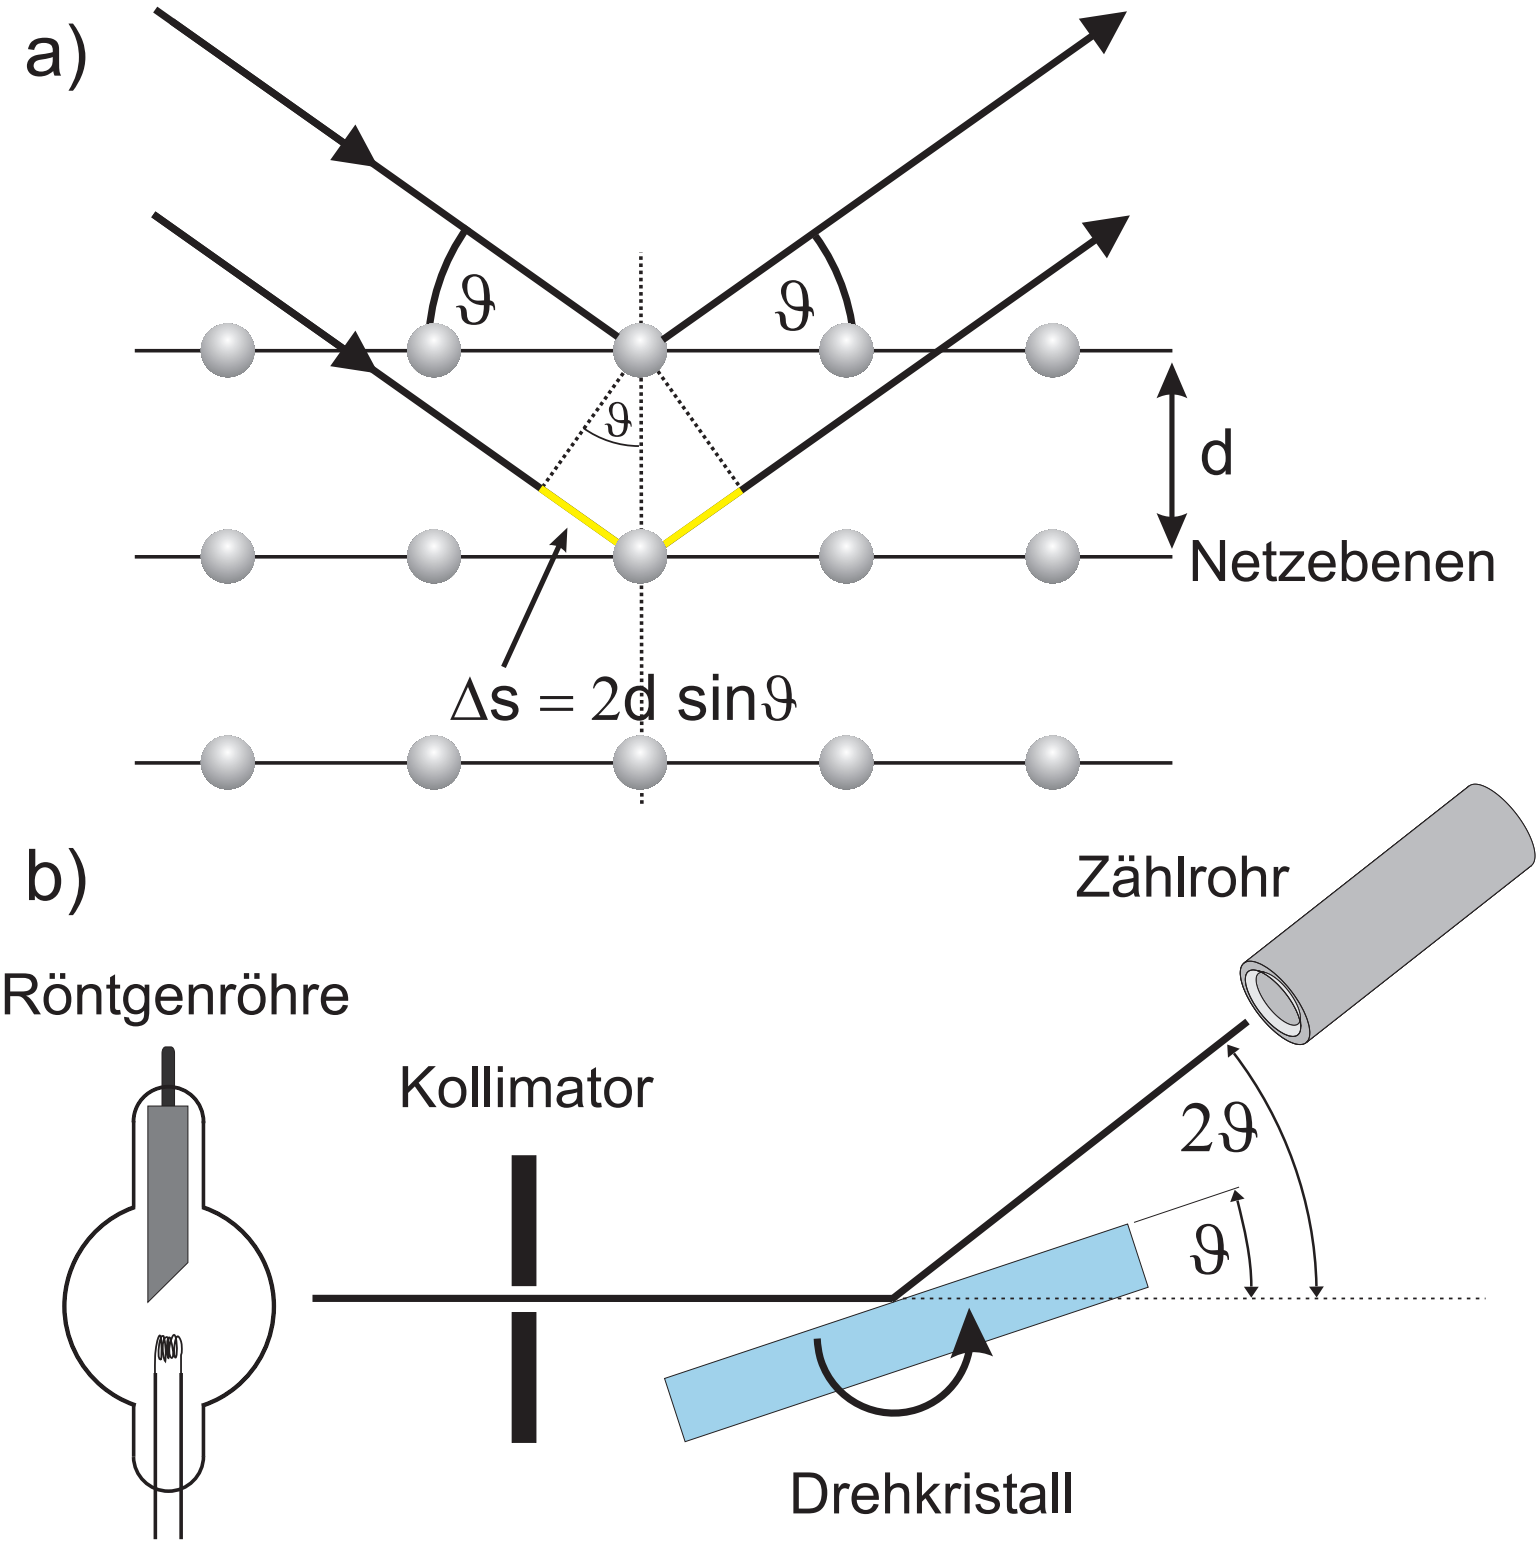
\includegraphics[width=.9\textwidth,trim={2cm 14cm 0.5cm 0},clip]{files/bragg_reflexion_drehkristall.png}
  \caption{Bragg-Reflexion von Röntenstrahlung an einem Kristall.}
  \label{fig:bragg_reflexion_drehkristall_a}
\end{figure}

Bei der sogenannten Drehkristallmethode wird diese Gesetzmäßigkeit angewandt. Dabei trifft Röntenstrahlung auf einen Kristall, welcher um die Achse senkrecht zu dieser gedreht wird. Welche Wellenlänge reflektiert wird, hängt dann gerade von der Winkelstellung des Kristalls ab. Die Intensität der reflektierten Strahlung kann dann mit einem Zählrohr gemessen und so Spektren wie in \abbref{fig:roentgenspektrum} aufgezeichnet werden. Ist der Drehkristall so justiert, dass gerade die Wellenlänge einer bekannten diskreten Linie reflektiert wird, lässt sich mit dem Bragg'schen Gesetz der Netzabstand $d$ berechnen.

\subsubsection*{Kristallstruktur}

Kristalle sind aus sich periodisch wiederholenden Elementarzellen aufgebaut, wie sie Beispielsweise in \abbref{fig:elementarzelle_nacl_reordered} zu sehen sind. Bei NaCl- und LiF-Kristallen sind die drei Gitterkonstanten, also die Seitenlängen $a$ einer Elementarzelle, gleich groß.

\begin{figure}[H]
  \centering
  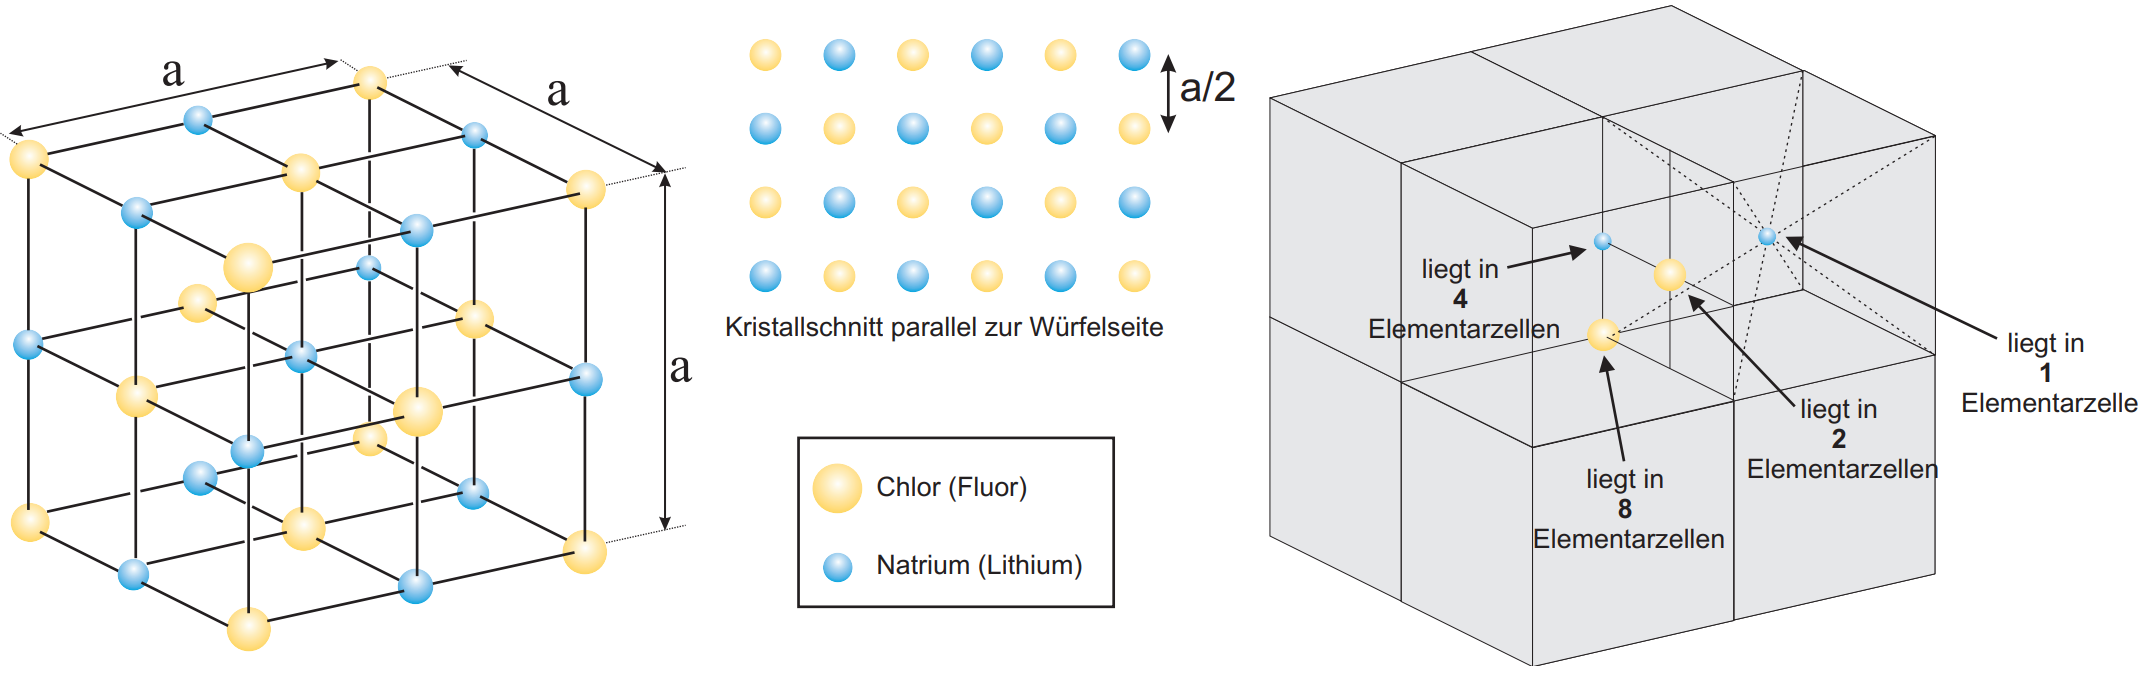
\includegraphics[width=\textwidth]{files/elementarzelle_nacl_reordered.png}
  \caption{Elementarzelle eines NaCl-Kristalls, deren periodische Anordnung, sowie der Kristallschnitt.}
  \label{fig:elementarzelle_nacl_reordered}
\end{figure}

Zur Ermittlung der Anzahl an Atomen, die einer Elementarzelle angehören, muss man beachten, zu wie vielen benachbarten Elementarzellen die Atome jeweils außerdem zählen. Dies ist ebenfalls in \abbref{fig:elementarzelle_nacl_reordered} dargestellt. Trägt ein Atom zu $x$ Elementarzellen bei, so zählt es für eine einzelne Elementarzelle nur zu $\flatfrac{1}{x}$. So lässt sich die Anzahl an Atomen am Beispiel der NaCl- (LiF-) Kristalle bestimmen.

\begin{table}[H]
  \centering
  \begin{tabular}{c|c|c|c||c|c}
    Element & Position & Beitrag zu x EZ & Beitrag zu einer EZ & Anzahl & Beitrag\\\hline
    Cl (F) & Ecken & $8$ & $\flatfrac{1}{8}$ & 8 & 1\\
    Cl (F) & Mitte Fläche & $2$ & $\flatfrac{1}{2}$ & 6 & 3\\
    Na (Li) & Mitte Kante & $4$ & $\flatfrac{1}{4}$ & 12 & 3\\
    Na (Li) & Mitte Zelle & $1$ & $\flatfrac{1}{1}$ & 1 & 1\\
  \end{tabular}
\end{table}

Aus den Beiträgen können ablesen, dass zu jeder Elementarzelle $4$ Chlor- (Fluor-) Atome und $4$ Natrium- (Lithium-) Atome, also $4$ NaCl- (LiF-) Moleküle, beitragen. Die Zahl $4$ geht bei der Berechnung der Avogadrokonstante wie folgt mit ein:
\begin{align}
  N_{A} = 4 \frac{V_{Mol}}{V}.
\end{align}
Dabei ist $V_{Mol}$ das Molvolumen eines einzelnen Moleküls und $V$ das Volumen einer Elementarzelle. Dieses lässt sich aus dem Netzabstand $d$, welcher hier $\flatfrac{a}{2}$ beträgt, berechnen. Somit gilt
\begin{align}
  N_A = 4 \frac{V_{Mol}}{(2d)^3} = 4 \frac{M_{Mol}}{\rho (2d)^3} = \frac{1}{2}\frac{M_{Mol}}{\rho d^3}.\label{eq:avogadro}
\end{align}

\subsection{Versuchsdurchführung}

Zur Durchführung der Messungen verwenden wir ein Röntgengerät, welches mit einem Zählrohr-Goniometer ausgestattet ist (\abbref{fig:goniometer}). Die Röntgenstrahlung wird durch eine Röntgenröhre mit Molybdänanode erzeugt und über einen Kollimator auf den Drehkristall fokussiert. Das Zählrohr am Goniometer dreht sich im Verhältnis 2:1 mit dem Drehkristall, sodass es immer genau die Strahlung, welche im Winkel $\vartheta$ reflektiert wird erfassen kann.

\begin{figure}[H]
  \centering
  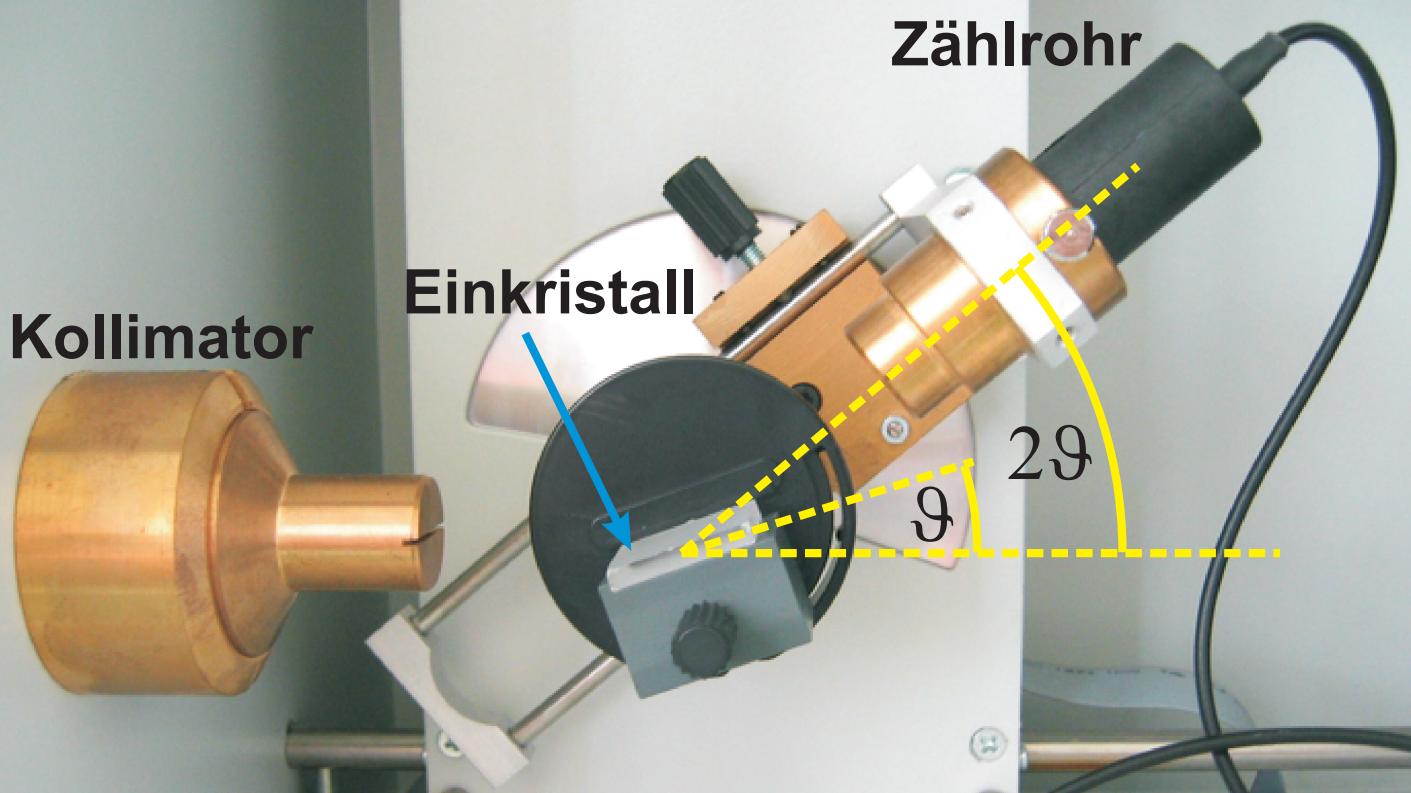
\includegraphics[width=.8\textwidth]{files/goniometer.png}
  \caption{Montierung des Drehkristalls und des Zählrohr-Goniometers im Winkelverhältnis 2:1.}
  \label{fig:goniometer}
\end{figure}

\textbf{Messung des Röntgenspektrums mit einem LiF-Kristall.} Bei einer Beschleunigungsspannung von $U = 35 \si{\kilo\volt}$, einem Strom von $I = 1\si{\milli\ampere}$ und einer Torzeit von $t = 5\si{\second}$ zeichnen wir das Röntgenspektrum in einem Winkelbereich von $3\si{\degree}$ bis $22\si{\degree}$ in $0.2\si{\degree}$-Schritten auf.

\textbf{Vermessen der $K_{\alpha}$ und $K_{\beta}$-Linien des Anodenmaterials.} Aus unseren Messdaten der vorherigen Aufgabe entnehmen wir die ungefähren Positionen der $K_{\alpha}$- und $K_{\beta}$-Linien. Mit den gleichen Einstellungen für Beschleunigungsspannung und Strom nehmen wir in deren Umgebung das Spektrum noch einmal in Winkelschritten von $0.1\si{\degree}$ und einer Torzeit von $20 \si{\second}$ auf.

\textbf{Zählrate als Funktion der Beschleunigungsspannung.} Bei einem festen Winkel von $7.5\si{\degree}$ Zeichnen wir die Zählrate für Beschleunigungsspannungen im Bereich von $20$ bis $35\si{\kilo\volt}$ in $1\si{\kilo\volt}$-Schritten jeweils über $20\si{\second}$ auf.

\textbf{Messung des Röntgenspektrums mit einem NaCl-Kristall.} Hier führen wir die Messung aus Aufgabe 1 noch einmal mit einem NaCl-Kristall in einem Winkelbereich von $3\si{\degree}$ bis $18\si{\degree}$ durch.
	
	
  
	%%%%%%%%%%%%%%%%%%%%%%%%%%%%%%%%%%%%%%%%%%%%%%%%%%%%%%%%%%%%%%%%%%%%%%%%
	\includepdf[scale=0.83,pages=1,pagecommand=\section{Messprotokoll}]{\protocolpdf}
  \includepdf[scale=0.83,pages=2-,pagecommand={\thispagestyle{plain}}]{\protocolpdf}
	
	%%%%%%%%%%%%%%%%%%%%%%%%%%%%%%%%%%%%%%%%%%%%%%%%%%%%%%%%%%%%%%%%%%%%%%%%
	\newpage\noindent
	\section{Auswertung}

\subsection{Bestimmung der Zeitkonstante eines RC-Glieds}

Wir verwenden die in Aufgabenteil 1 gemessenen Halbwertszeiten, um die Zeitkonstante nach Gleichung \eqref{eq:zeitkonst} zu berechnen. Den theoretischen Wert der Zeitkonstante ermitteln wir anhand der Formel $\tau = RC$ mit dem Widerstand $R$ und der Kapazität $C$. Die resultate der Berechnungen für alle vier Konfigurationen der RC-Schaltung sind \tabref{tab:a1_zeitkonst} zu entnehmen.

\begin{table}[h]
  \centering
  \begin{tabular}{| c | c | c | c | c | c |}
      \hline
      $C\ [\si{\nano\farad}]$ & $R\ [\si{\kilo\ohm}]$ & $f\ [\si{\hertz}]$ & $\tau_{\text{theo}}\  [\si{\second}]$ & $\tau_{\text{exp}}\ [\si{\second}]$ & Abw. \\
      \hline
      $470 \pm 47$ & $1.00 \pm 0.05$ & $165 \pm 1$ & $(47 \pm 6) \times 10^{-5}$ & $(43 \pm 15) \times 10^{-5}$ & $0.25\sigma$ \\
      \hline
      $4.70 \pm 0.47$ & $10.00 \pm 0.50$ & $165 \pm 1$ & $(4.7 \pm 0.6) \times 10^{-5}$ & $(6.49 \pm 0.15) \times 10^{-5}$ & $3.29\sigma$ \\
      \hline
      $47.00 \pm 4.70$ & $1.00 \pm 0.05$ & $165 \pm 1$ & $(4.7 \pm 0.6) \times 10^{-5}$ & $(4.91 \pm 0.15) \times 10^{-5}$ & $0.38\sigma$ \\
      \hline
  \end{tabular}
  \caption{Messwerte und berechnete Größen}
  \label{tab:a1_zeitkonst}
\end{table}

\abbref{fig:aufgabe1_rc_signalverlauf} zeigt exemplarisch den Spannungsverlauf für die letzte angegebene Schaltungskonfiguration. 


\begin{figure}[H]
  \centering
  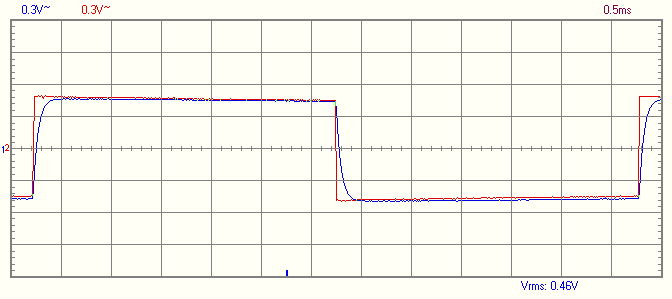
\includegraphics[width=.8\textwidth]{files/aufgabe1_rc_signalverlauf.png}
  \caption{Spannungsverlauf am Oszilloskop des RC-Glieds für $C = 47\si{\nano\farad}$, $R = 1 \si{\kilo\ohm}$. In Rot dargestellt die Eingangsspannung $U_E$, in Blau die Ausgangsspannung $U_C$, abgenommen über den Kondensator.}
  \label{fig:aufgabe1_rc_signalverlauf}
\end{figure}

\subsection{RC-Glied als Integrator und Differentiator}

Wie bereits dem Versuchsprotokoll zu entnehmen können wir beim Aufbau der RC-Schaltung als Integrator beobachten, dass sich das Ausgangssignal bei Erhöhung des Widerstandes immer stärker dem Integral des Eingangssignals annähert. So formt ein eingehendes Rechteckssignal eine Dreiecksfunktion als Ausgangssignal, aus einem eingehenden Dreieckssignal ergibt sich ein Sinussignal, wie in \abbref{fig:aufgabe2_integral_dreieck} zu sehen.

\begin{figure}[H]
  \centering
  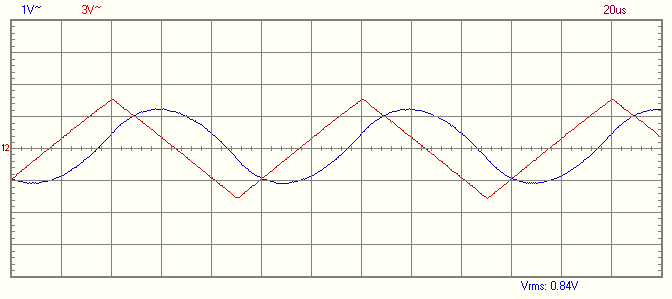
\includegraphics[width=.8\textwidth]{files/aufgabe2_integral_dreieck.png}
  \caption{Spannungsverlauf beim Betrieb der RC-Schaltung als Integrator. In Rot dargestellt die dreiecksförmige Eingangsspannung $U_E$, in Blau die Ausgangsspannung $U_C$, abgenommen über den Kondensator.}
  \label{fig:aufgabe2_integral_dreieck}
\end{figure}

Ähnliche Beobachtungen können wir beim Betrieb des RC-Glieds als Differentiator machen. Bei Justierung des Widerstandes ergibt sich hierbei beispielsweise aus einem eingehenden Dreieckssignal ein ausgehendes Rechteckssignal, siehe \abbref{fig:aufgabe2_differentiator_dreieck}. Geben wir durch den Funktiongenerator ein Signal in der Form einer Gauß'schen Normalverteilung ein, so ergibt sich auch hiervon die entsprechende Ableitung, zu sehen in \abbref{fig:aufgabe2_differentiator_gauss}.


\begin{figure}[H]
  \centering
  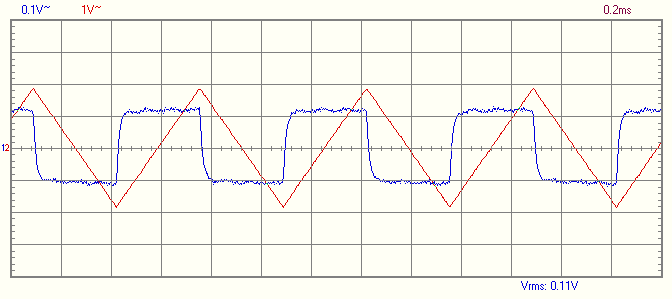
\includegraphics[width=.8\textwidth]{files/aufgabe2_differentiator_dreieck.png}
  \caption{Spannungsverlauf beim Betrieb der RC-Schaltung als Differentiator. In Rot dargestellt die dreiecksförmige Eingangsspannung $U_E$, in Blau die Ausgangsspannung $U_R$, abgenommen über den Widerstand.}
  \label{fig:aufgabe2_differentiator_dreieck}
\end{figure}

\begin{figure}[H]
  \centering
  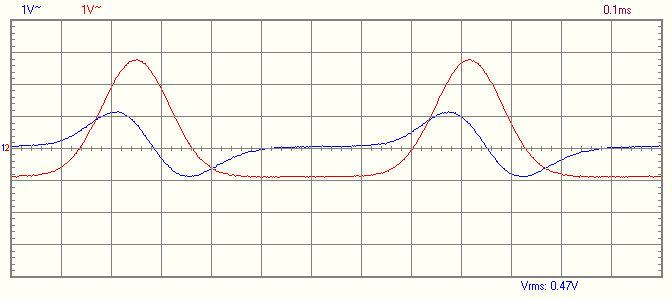
\includegraphics[width=.8\textwidth]{files/aufgabe2_differentiator_gauss.png}
  \caption{Spannungsverlauf beim Betrieb der RC-Schaltung als Differentiator. In Rot dargestellt die Eingangsspannung $U_E$, in Blau die Ausgangsspannung $U_R$, abgenommen über den Widerstand.}
  \label{fig:aufgabe2_differentiator_gauss}
\end{figure}


\subsection{Frequenz- und Phasengang eines RC-Glied}

In diesem Teil der Auswertung bestimmen wir aus dem aufgezeichneten Frequenzgängen eines Tief- und Hochpassfilters die Grenzfrequenz bestimmen. Wie in den theoretischen Grundlagen erklärt, ist die Grenzfrequenz der Filterschaltung dadurch zu erkennen, dass bei ihr die Amplitude um den Faktor $\flatfrac{1}{\sqrt{2}}$ abgefallen ist. Mit der \textit{Curser}-Funktion des Oszilloskops können wir damit eine Grenzfrequenz von $(9.46 \pm 0.02)\si{\hertz}$ für den Tiefpassfilter und eine Grenzfrequenz von $(3.31 \pm 0.02) \si{\hertz}$ für den Hochpassfilter ablesen. Die untenstehenden Abbildungen zeigen noch einmal die Frequenzgänge des Tiefpassfilters (\ref{fig:aufgabe3_tiefpass}) und Hochpassfilters (\ref{fig:aufgabe3_hochpass}), jeweils mit dem Cursor an der Grenzfrequenz.


\begin{figure}[H]
  \centering
  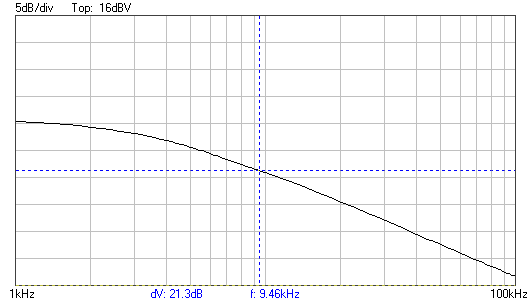
\includegraphics[width=.8\textwidth]{files/aufgabe3_tiefpass.png}
  \caption{Frequenzgang des Tiefpassfilters mit Cursor bei Grenzfrequenz}
  \label{fig:aufgabe3_tiefpass}
\end{figure}

\begin{figure}[H]
  \centering
  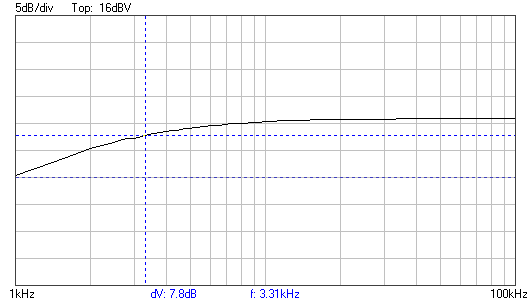
\includegraphics[width=.8\textwidth]{files/aufgabe3_hochpass.png}
  \caption{Frequenzgang des Hochpassfilters mit Cursor bei Grenzfrequenz}
  \label{fig:aufgabe3_hochpass}
\end{figure}

Neben der Aufzeichnung des Frequenzgangs haben wir für den Hochpassfilter zusätzlich den Phasengang manuell vermessen. Die Phase $\varphi$ ist in \abbref{fig:phaseshift_hp_fit} über der Frequenz aufgetragen. Die Grenzfrequenz bestimmen wir nun durch Ablesen Frequenz bei einer Phase von $45\si{\degree}$. Die Phase zeigt, abhängig von der Frequenz, einen logarithmisch abfallenden Verlauf auf. Um den Wert bei $45\si{\degree}$ interpolieren zu können fitten wir eine abfallende Exponentialfunktion der Form
\begin{align}
  f(x; A,\lambda,c) = A \cdot \e{- \lambda x} + c
\end{align}
an die Datenpunkte an. Die optimierten Werte der Parameter sind ebenfalls der \abbref{fig:phaseshift_hp_fit} zu entnehmen.


\begin{figure}[H]
  \centering
  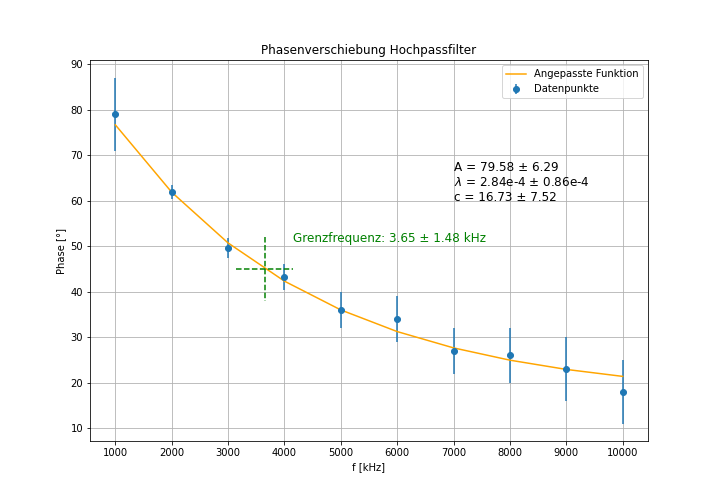
\includegraphics[width=.8\textwidth]{files/phaseshift_hp_fit.png}
  \caption{Phasengang des Hochpassfilters mit exponentiellem Fit und Grenzfrequenz bei $45\si{\degree}$.}
  \label{fig:phaseshift_hp_fit}
\end{figure}


Durch elementares Umformen bestimmen wir die Umkehrfunktion von $f$, um damit die Grenzfrequenz berechnen zu können. Für diese gilt
\begin{align}
  f^{-1}(\varphi; A, \lambda, c) = - \frac{1}{\lambda} \ln(\frac{\varphi - c}{A}) = f_{\mathrm{Grenz}}.
\end{align}
Nach der gauß'schen Fehlerfortpflanzung gilt für der Fehler des damit berechneten Wertes
\begin{align}
  \Delta f_{\mathrm{Grenz}} = \sqrt{\qty(\frac{1}{\lambda A} \ln(\frac{\varphi - c}{A}) \cdot \Delta A)^{2} + \qty(\frac{1}{\lambda^2} \ln(\frac{\varphi - c}{A}) \cdot \Delta \lambda)^{2} + \qty(\frac{1}{\lambda(\varphi - c)} \cdot \Delta c)^{2}}.
\end{align}

Damit können wir aus der Funktion eine Grenzfrequenz von
\begin{align}
  f_{\mathrm{Grenz}} = (3.65 \pm 1.48) \si{\kilo\hertz}
\end{align}
interpolieren. Diese ist ebenfalls in Grün in \abbref{fig:phaseshift_hp_fit} markiert. Von der zuvor vermessenen Grenzfrequenz weicht diese um etwa $2.47\sigma$ ab, was innerhalb des $3\sigma$-Bereichs noch als eine nicht signifikant Abweichung angesehen werden kann.
	
	
	
	%%%%%%%%%%%%%%%%%%%%%%%%%%%%%%%%%%%%%%%%%%%%%%%%%%%%%%%%%%%%%%%%%%%%%%%%
	\newpage\noindent
	\section{Zusammenfassung und Diskussion}

In Versuch 234 beschäftigen wir uns mit der Untersuchung der Spektren verschiedener Lichtquellen. Hier unterscheiden wir zwischen Temperaturstrahlern und Nichttemperaturstrahlern. Temperaturstrahler, wie beispielsweise eine Glühlampe, basieren auf dem Phänomen, dass jeder Körper, dessen Temperatur größer als $0\si{\kelvin}$ ist, elektromagnetische Strahlung abstrahlt, deren Intensitätsverteilung abhängig von der Wellenlänge dem Planck'schen Strahlungsgesetz folgt. Bei den Nichttemperaturstrahlern ist die Erzeugung von Licht entweder auf Anregung von Atomzuständen, zum Beispiel bei einer Natriumdampflampe, oder der Rekombination von Elektron-Loch-Paaren in Halbleitern, also LEDs, zurückzuführen.

Im ersten Versuchsteil untersuchten wir das Spektrum des wohl bekanntesten Temperaturstrahlers, der Sonne. Mit einem Gitterspektroskop nahmen wir das Spektrum des Tageslichts einmal direkt und einmal durch ein Fenster auf. Wir konnten beobachten, dass es sich um ein kontinuierliches Spektrum handelt, wie es von Temperaturstrahlern zu erwarten ist. 

\begin{figure}[H]
  \centering
  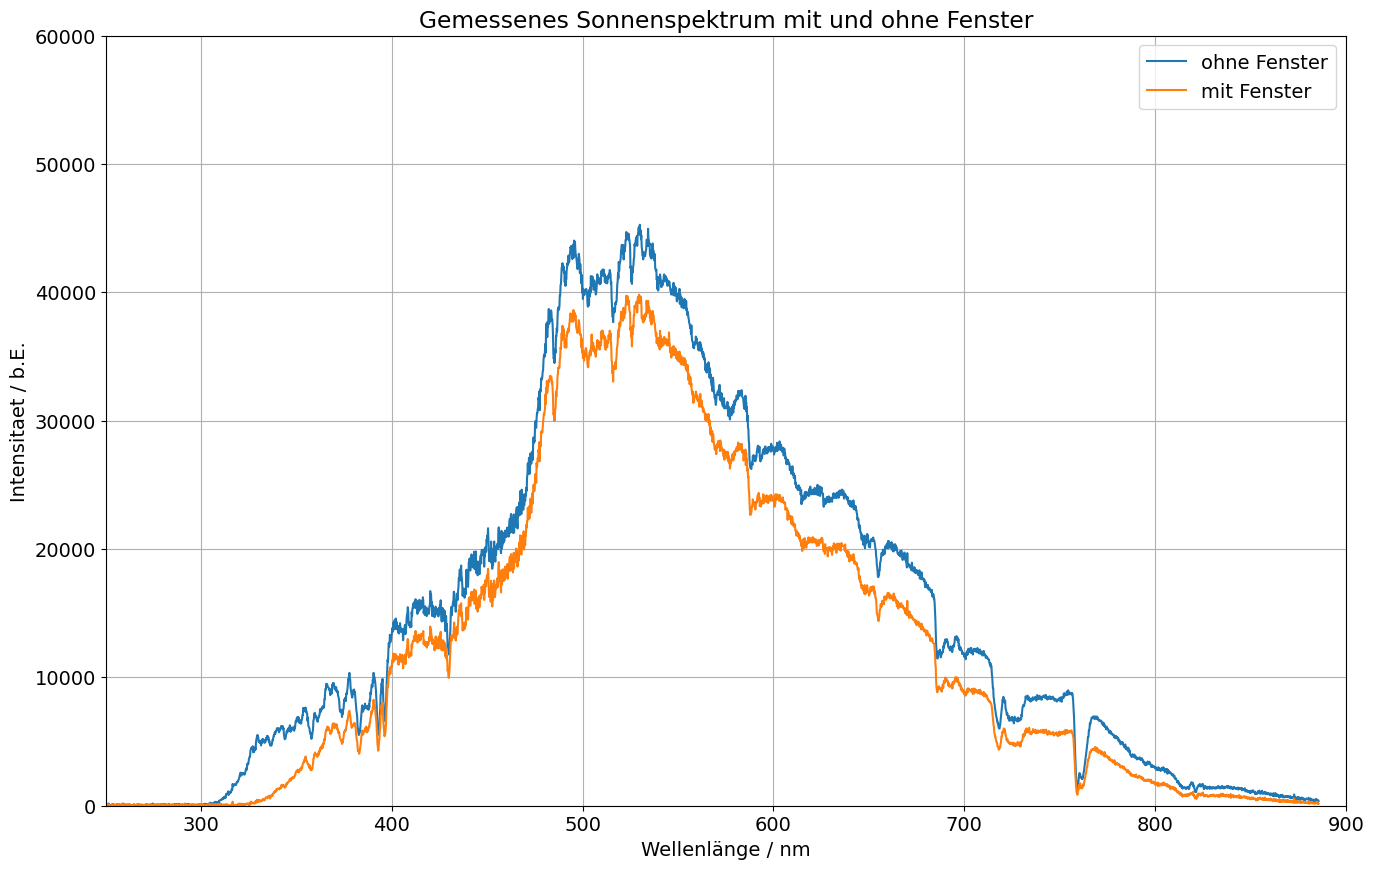
\includegraphics[width=.9\textwidth]{files/plots/himmel_m_o_g.png}
  \caption{Tageslichtspektrum direkt (blau) und durch Fensterglas (orange).}
  \label{fig:himmel_m_o_g_zsmf}
\end{figure}


Im Vergleich des Spektrums durch das Fenster mit dem, das direkt aufgezeichnet wurde, konnten wir beobachten, dass durch die Scheibe über den gesamten Wellenlängenbereich hinweg die Intensität des Lichts durch die Absorption der Glasscheibe abgeschwächt wird. Bei genauerer Betrachtung der Absorption konnten wir sehen, dass diese im Bereich von Wellenlängen unter $400\si{\nano\meter}$, also im nicht-sichtbaren UV-Bereich, am höchsten und im Bereich des sichtbaren Lichts am niedrigsten ist.

Die vielen im Spektrum deutlich sichtbaren lokalen Minima sind durch die Absorption von Licht bestimmter Wellenlängen in den Atmosphärenschichten der Sonne und der Erde zu erklären. Diese Absorptionslinien, genannt \glqq{}Fraunhoferlinien\grqq{} sind speziellen Wellenlängen zugeordnet, welche wir mit den Positionen der Linien in unsren aufgezeichneten Spektrum verglichen. Die Werte sind, mit der jeweiligen Abweichung vom Literaturwert in \tabref{tab:fraunhofer_vergleich_zsmf} zusammengefasst. Als Fehler für die beobachteten Wellenlängen sind wir jeweils von $\pm 1\si{\nano\meter}$ ausgegangen.

\begin{table}[h]
  \centering
  \caption{Vergleich der erwarteten und gemessenen Wellenlängen der Fraunhofer- und Balmerlinien}
  \vspace*{0.5em}
  \begin{tabular}{c|c|c|c}
      \hline
      Linie & Literaturwert [nm] & Abgelesener Wert [nm] & Abweichung [$\sigma$] \\
      \hline
      K  & 393.4 & 393.0 & 0.4 \\
      H  & 396.8 & 396.1 & 0.7 \\
      G  & 430.8 & 429.8 & 1.0 \\
      F  & 486.1 & 485.2 & 0.91 \\
      b1 & 518.4 & 516.7 & 1.7 \\
      E  & 527.0 & 526.2 & 0.8 \\
      D3 & 587.6 & 588.4 & 0.8 \\
      D2 & 589.0 & 589.0 & 0.0 \\
      D1 & 589.6 & 589.7 & 0.11 \\
      C  & 656.3 & 655.0 & 1.3 \\
      B  & 686.7 & 686.7 & 0.0 \\
      A  & 759.4 & 759.4 & 0.0 \\
      \hline\hline
      $\mathrm{H}_{\alpha}$ & 656.3 & 655.0 & 1.3\\
      $\mathrm{H}_{\beta}$ & 486.1 & 485.2 & 0.91\\
      $\mathrm{H}_{\gamma}$ & 434.0 & 433.4 & 0.61\\
      $\mathrm{H}_{\delta}$ & 410.1 & 409.5 & 0.61\\
      \hline
  \end{tabular}
  \label{tab:fraunhofer_vergleich_zsmf}
\end{table}

Unter anderem als lokale Minima im Sonnenlichtspektrum zu beobachten sind die Linien der Balmerserie, welche auf Anregungen in Wasserstoffatom zurückzuführen sind. Die beobachteten Positionen der $H_{\alpha}-, H_{\beta}-, H_{\gamma}-, H_{\delta}-$Linien der Balmerserie verglichen wir ebenfalls mit den Literaturwerten, zusammengefasst in derselben Tabelle.

Insgesamt ist die Abweichung der beobachteten Absorptionslinien von den Literaturwerten sehr gering. Die dennoch sichtbaren Unterschieden sind vermutlich zu Großteilen auf das wolkige Wetter am Versuchstag, sowie Störungen und Reflexionen durch die umliegenden Gebäude zurückzuführen.

Im darauf folgenden Versuchsteil betrachteten wir qualitativ die Spektren verschiedener Lichtquellen. Hierunter untersuchten wir das Licht verschiedenfarbiger LEDs, eines Lasers und einer Energiesparlampe als Beispiele für Nichttemperaturstrahler, sowie das einer Glühlampe als ein klassisches Beispiel für einen Temperaturstrahler. Wie in der Theorie beschrieben, konnten wir beobachten, dass die LEDs, der Laser und die Energiesparlampe diskrete Spektren aufweisen. Dabei basiert die Erzeugung von weißem Licht bei den weißen LEDs und der Energiesparlampe auf verschiedenen Methoden. Die Glühlampe wies ein kontinuierliches Spektrum auf, von welchem große Teile außerhalb des sichtbaren Wellenlängenbereichs lagen. Dies zeigte auch, dass diese im Vergleich zu den anderen Lichtquellen viel weniger energieeffizient ist.

Im abschließenden großen Versuchsblock setzen wir uns mit dem Spektrum einer Natriumdampflampe auseinander. Als Beispiel für eine Gasentladungslampe weist diese ein diskretes Spektrum auf, welches durch eine Vielzahl an Spektrallinien über den gesamten beobachteten Wellenlängen charakterisiert ist. Wir betrachteten zunächst das Spektrum in einem Wellenlängenbereich von $350$ bis $550\si{\nano\meter}$. Hier sind Spektrallinien mit geringer Intensität zu beobachten. Wir notierten die Wellenlängen aller gut sichtbarer Linien für den späteren Vergleich. Im Bereich zwischen $590$ und $600\si{\nano\meter}$ befindet sich im Natriumspektrum die markante D-Linie. Auch die Wellenlänge dieser Linie selbst, sowie die Wellenlängen einiger umliegender Linien notierten wir uns. Zuletzt zeichneten wir noch die Wellenlängen einiger markanter Linien im oberen Wellenlängenbereich von $650$ bis $850\si{\nano\meter}$ auf.

Zum Vergleich der beobachteten mit den theoretisch vorhersagten Positionen der Spektrallinien betrachteten wir dann die Übergänge $md \to 3p$ der 1. Nebenserie, die Übergänge $ms \to 3p$ der 2. Nebenserie, sowie die $mp \to 3s$ der Hauptserie. Die Energie $E_{3p}$, welche wir für die Berechnungen der Wellenlängen der Übergänge zum $3p$-Zustand benötigen, bestimmten wir auf einen Wert von
\begin{align}
  E_{3p} = -3.0279 \pm 0.0019\si{\electronvolt}.
\end{align}

Mit diesem bestimmten wir anhand der Formel $\lambda_m \approx \flatfrac{hc}{\qty(\frac{E_{Ry}}{m^2} - E_{3p})}$ für die Quantenzahlen $m=3,\dots,12$ die erwarteten Wellenlängen der Spektrallinien. Diese sind in \tabref{tab:wellenlaengen_1ns_zsmf} zusammen mit den von uns beobachteten Wellenlängen, welche wir diesen zuordnen konnten, aufgelistet.

\begin{table}[H]
  \centering
  \caption{Vergleich der berechneten und gemessenen Wellenlängen der 1. Nebenserie $md \to 3p$.}
  \vspace*{0.5em}
  \begin{tabular}{c c c c}
      \hline
      $m$ & $\lambda_{\text{theo.}}$ [nm] & $\lambda_{\text{beob.}}$ [nm] & Abweichung \\
      \hline
      3  & $817.7 \pm 1.000$ & $817.7 \pm 1$ & 0.01$\sigma$ \\
      4  & $569.4 \pm 0.5$ & $567.1 \pm 1$ & 2.03$\sigma$ \\
      5  & $499.2 \pm 0.4$ & $496.9 \pm 2$ & 1.13$\sigma$ \\
      6  & $467.9 \pm 0.4$ & $469.2 \pm 1$ & 1.28$\sigma$ \\
      7  & $450.8 \pm 0.4$ & $450.0 \pm 1$ & 0.77$\sigma$ \\
      8  & $440.4 \pm 0.3$ & $438.1 \pm 1$ & 2.20$\sigma$ \\
      9  & $433.5 \pm 0.3$ & $432.6 \pm 1$ & 0.88$\sigma$ \\
      10 & $428.7 \pm 0.3$ & $429.2 \pm 1$ & 0.46$\sigma$ \\
      11 & $425.3 \pm 0.3$ & $426.0 \pm 1$ & 0.72$\sigma$ \\
      12 & $422.7 \pm 0.3$ & $423.1 \pm 1$ & 0.44$\sigma$ \\
      \hline
  \end{tabular}
  \label{tab:wellenlaengen_1ns_zsmf}
\end{table}

Wir können sehen, dass die Abweichung bei den meisten Linien unter einem $\sigma$ liegt. Bei den Vergleichen mit einer signifikanteren Abweichung kann es durchaus sein, dass den theoretisch vorhersagten Linien falsche beobachtete Linien zugeordnet wurden.

Analog gingen wir für die 2. Nebenserie vor. Für die Berechnung der Wellenlängen benötigen wir hierbei zusätzlich den Korrekturterm $\Delta_s$. Um diesen zu bestimmen, berechneten wir zunächst die Energie des Zustandes $3s$ zu
\begin{align}
  E_{3s} = (-5.127 \pm 0.005)\si{\electronvolt},
\end{align}
und daraus wiederum den Korrekturterm
\begin{align}
  \Delta_s = 1.3711 \pm 0.0007.
\end{align}

Dieser ging dann mit in die Formel $\lambda_m \approx \flatfrac{hc}{\qty(\frac{E_{Ry}}{(m - \Delta_s)^2} - E_{3p})}$ mit ein, um die Wellenlängen für die Quantenzahlen $m=4,\dots,9$ zu bestimmen. Die Resultate sind in \tabref{tab:wellenlaengen_2ns_zsmf} noch einmal wiedergegeben. Da diese außerhalb des untersuchten Bereichs liegt, konnten wir der Spektrallinie für den Übergang $3s\to3p$ keine beobachtete Wellenlänge zuordnen. Bei allen weiteren sehen wir erneut, dass die Abweichung zwischen den jeweils zugeordneten Linien weitestgehend gering ausfällt. Lediglich die Linie der Quantenzahl $m=7$ weicht etwas stärker ab, was möglicherweise auf eine falsche Zuordnung zurückzuführen ist.

\begin{table}[H]
  \centering
  \caption{Vergleich der berechneten und gemessenen Wellenlängen der 2. Nebenserie $ms \to 3p$.}
  \vspace*{0.5em}
  \begin{tabular}{c c c c}
      \hline
      $m$ & $\lambda_{\text{theo.}}$ [nm] & $\lambda_{\text{beob.}}$ [nm] & Abweichung \\
      \hline
      4  & $1170.366 \pm 1.302$ & -     & -     \\
      5  & $621.527 \pm 0.692$  & $622.34 \pm 1$ & $0.67\sigma$ \\
      6  & $518.112 \pm 0.577$  & $517.50 \pm 1$ & $0.53\sigma$ \\
      7  & $477.124 \pm 0.531$  & $474.00 \pm 1$ & $2.76\sigma$ \\
      8  & $456.100 \pm 0.508$  & $454.40 \pm 1$ & $1.52\sigma$ \\
      9  & $443.719 \pm 0.494$  & $445.30 \pm 1$ & $1.42\sigma$ \\
      \hline
  \end{tabular}
  \label{tab:wellenlaengen_2ns_zsmf}
\end{table}

Noch einmal nach dem gleichen Schema berechneten wir abschließend die erwarteten Wellenlängen der Hauptserie. Hierzu bestimmten wir zunächst den Korrekturterm
\begin{align}
  \Delta_p = 0.8803 \pm 0.0007.
\end{align}

Die berechneten Wellenlängen für die Quantenzahlen $m=4,5$ sind in \tabref{tab:wellenlaengen_hs_zsfm} zu finden. Da beide unter $350\si{\nano\meter}$ liegen und damit außerhalb des von uns beobachteten Bereichs, können wir diese nicht vergleichen.

\begin{table}[H]
  \centering
  \caption{Berechnete Wellenlängen der Hauptserie $mp \to 3s$.}
  \vspace*{0.5em}
  \begin{tabular}{c c c c}
      \hline
      $m$ & $\lambda_{\text{theo.}}$ [nm] & $\lambda_{\text{beob.}}$ [nm] & Abweichung \\
      \hline
      4  & $332.4 \pm 0.6$ & -     & -     \\
      5  & $286.6 \pm 0.5$  & - & - \\
      \hline
  \end{tabular}
  \label{tab:wellenlaengen_hs_zsfm}
\end{table}

Im letzten Teil der Auswertung passten wir die Funktion
\begin{align}
  f(m;E_{Ry}, E_{3p}, \Delta_{d(s)}) = \frac{hc}{\frac{E_{Ry}}{(m - \Delta_{d(s)})^2} - E_{3p}} = \lambda_m
\end{align}
abhängig von der Quantenzahl $m$ an die Werte der beobachteten Wellenlängen der 1. und 2. Nebenserie an, um die Parameter $E_{Ry}, E_{3p}$ und $\Delta_{d}$ bzw. $\Delta_{s}$ zu bestimmen. Die optimierten Parameter aus der Anpassung an die 1. Nebenserie sind in \tabref{tab:fit_1ns_vergl} zusammengefasst. Zusätzlich ist hier auch die Abweichung zu den Werten, welche wir im vorherigen Aufgabenteil berechnet hatten, angegeben.


\begin{table}[H]
  \centering
  \caption{Werte der Parameter, bestimmt durch Fit an die Wellenlängen der 1. Nebenserie, und Vergleich.}
  \vspace*{0.5em}
  \begin{tabular}{c c c c}
      \hline
      Parameter & Wert & Fehler & Abw. vom zuvor berechneten Wert \\
      \hline
      $E_{Ry}$  & $-13.0 \si{\electronvolt}$ & $0.5\si{\electronvolt}$ & $1.53\sigma$ \\
      $E_{3p}$  & $-3.023\si{\electronvolt}$  & $0.006\si{\electronvolt}$ & $0.75\sigma$ \\
      $\Delta_{d}$  & $0.07$  & $0.05$ & - \\
      \hline
  \end{tabular}
  \label{tab:fit_1ns_vergl}
\end{table}

Die reduzierte $\chisq$-Summe liegt mit einem Wert von $\chisqrd = 1.50$ nahe am optimalen Wert $1$. Somit können wir bei diesen Fit die Beschreibung der Daten durch das gegebene Modell bzw. die gegebene Funktion allgemein als gut Bewerten. Dies ist auch durch relativ geringen Unsicherheiten der optimierten Parameter zu erkennen. Die Fitwahrscheinlichkeit liegt allerdings nur bei $16.0\%$. Wie aber auch in der Praktikumsanleitung angeführt, liegt dies daran, dass $\Delta_d$ nur eine empirische Näherungsformel ist und in Wirklichkeit auch schwach von der Hauptquantenzahl $n$ abhängt. Die Abweichungen von den zuvor berechneten Werten sind mit Werten von um einem $\sigma$ nicht ausschlaggebend.

Im Anschluss führten wir noch einen Fit an die Wellenlängen der 2. Nebenserie durch. Hierbei optimierten wir anstatt dem Korrekturterm $\Delta_d$, den Term $\Delta_s$, welchen wir auch bereits im vorherigen Aufgabenteil verwendet hatten. Die optimierten Werte der Parameter sind, in gleicher Form wie zuvor, in \tabref{tab:fit_2ns_vergl} zusammengefasst.

\begin{table}[H]
  \centering
  \caption{Werte der Parameter, bestimmt durch Fit an die Wellenlängen der 2. Nebenserie, und Vergleich.}
  \vspace*{0.5em}
  \begin{tabular}{c c c c}
      \hline
      Parameter & Wert & Fehler & Abw. vom zuvor berechneten Wert \\
      \hline
      $E_{Ry}$  & $-11.6 \si{\electronvolt}$ & $2.1\si{\electronvolt}$ & $1.01\sigma$ \\
      $E_{3p}$  & $-3.01\si{\electronvolt}$  & $0.04\si{\electronvolt}$ & $0.68\sigma$ \\
      $\Delta_{s}$  & $1.62$  & $0.25$ & $1.03\sigma$ \\
      \hline
  \end{tabular}
  \label{tab:fit_2ns_vergl}
\end{table}

Für diesen Fit hatten wir nur halb so viele Datenpunkte wie im vorherigen Fit zur Verfügung. Dies spiegelt sich auch in den nun sehr hohen Ungenauigkeiten der optimierten Parameter, sowie der Bewertung der Güte des Fits wider. Die reduzierte $\chisq$-Summe beträgt hier $\chisqrd = 4.28$, was für eine schlechte Beschreibung der Daten durch das verwendete Modell steht. Mit gerade einmal $1\%$ ist auch hier die Fitwahrscheinlichkeit sehr schlecht, was erneut auf das zum vorherigen Fit beschriebene Problem zurückzuführen sein könnte. Die Abweichungen zu den zuvor berechneten Werten der optimierten Parameter sind in diesem Fit geringer als im vorherigen, was allerdings daran liegt, dass die Unsicherheiten hier deutlich größer sind.


	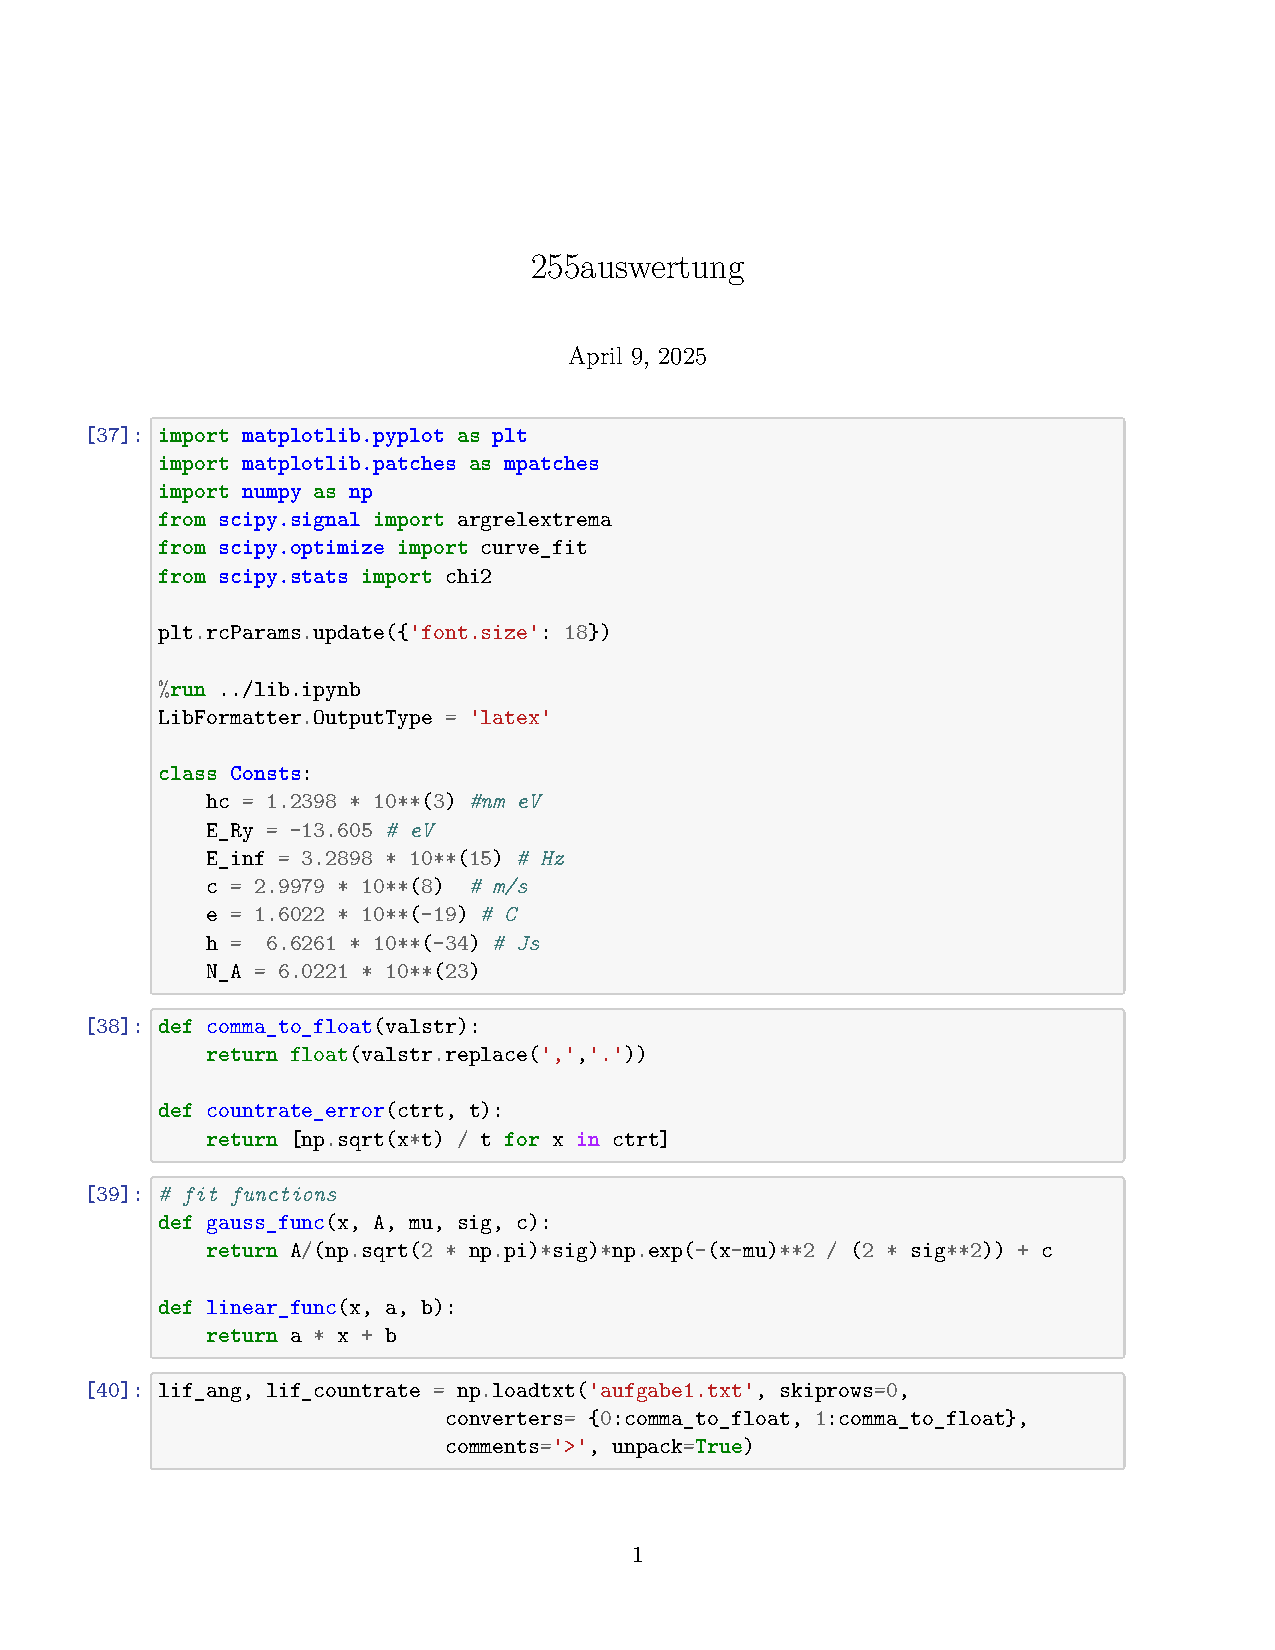
\includepdf[scale=0.95,pages=1,pagecommand=\section*{Python Code, Hauptprogramm}]{files/255auswertung.pdf}
	\includepdf[scale=0.95,pages=2-,pagecommand={\thispagestyle{plain}}]{files/255auswertung.pdf}

	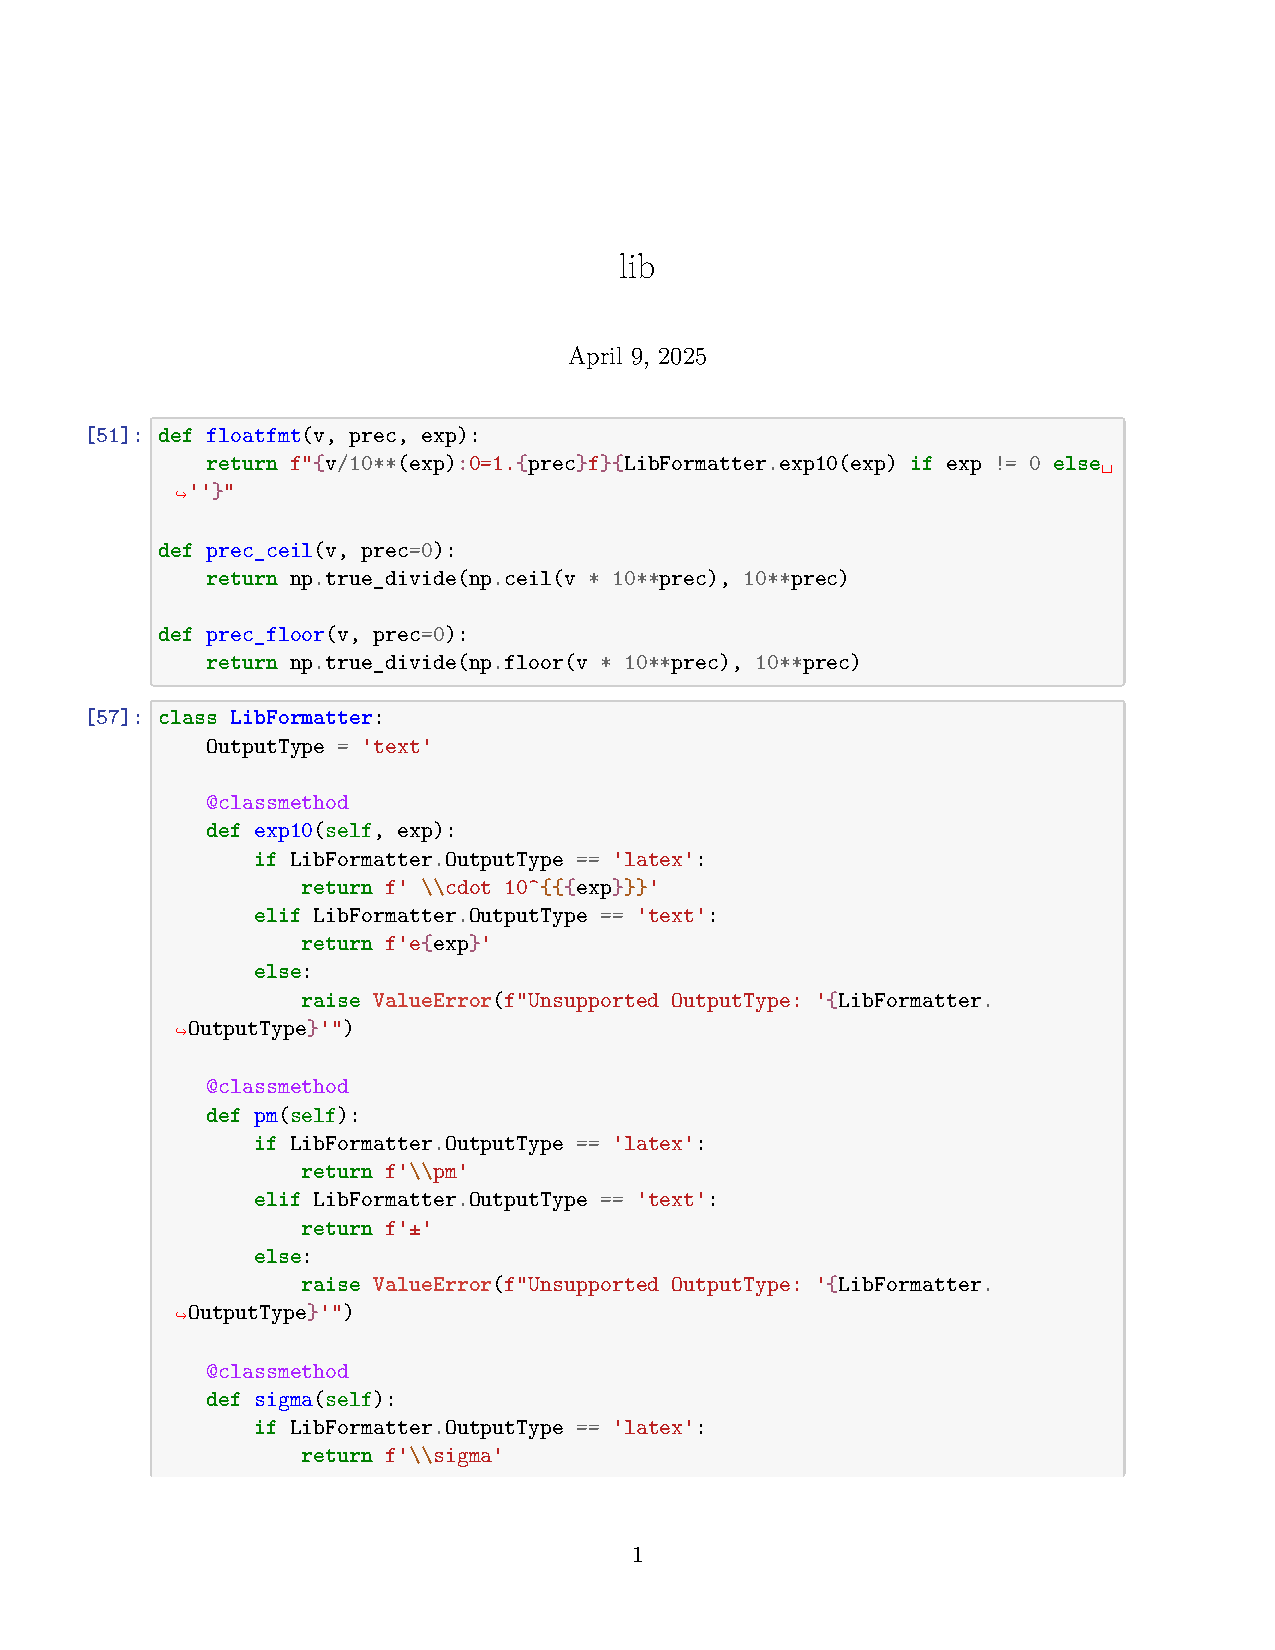
\includepdf[scale=0.95,pages=1,pagecommand=\section*{Python Code, Bibliothek}]{files/lib.pdf}
	\includepdf[scale=0.95,pages=2-,pagecommand={\thispagestyle{plain}}]{files/lib.pdf}
	
	
	
\end{document}

